\subsection{Places}\label{sec:places}
The Places\autocite{Places365} dataset is intended for scene understanding and scene recognition tasks. 
It is an MIT Big Data Initiative, which has gathered and catalogued more than 10M images comprising 400+ unique scene categories.
The categories include highways, pantries, fire stations, landfills, rainforests and much more.
\begin{figure}[H]
    \centering
    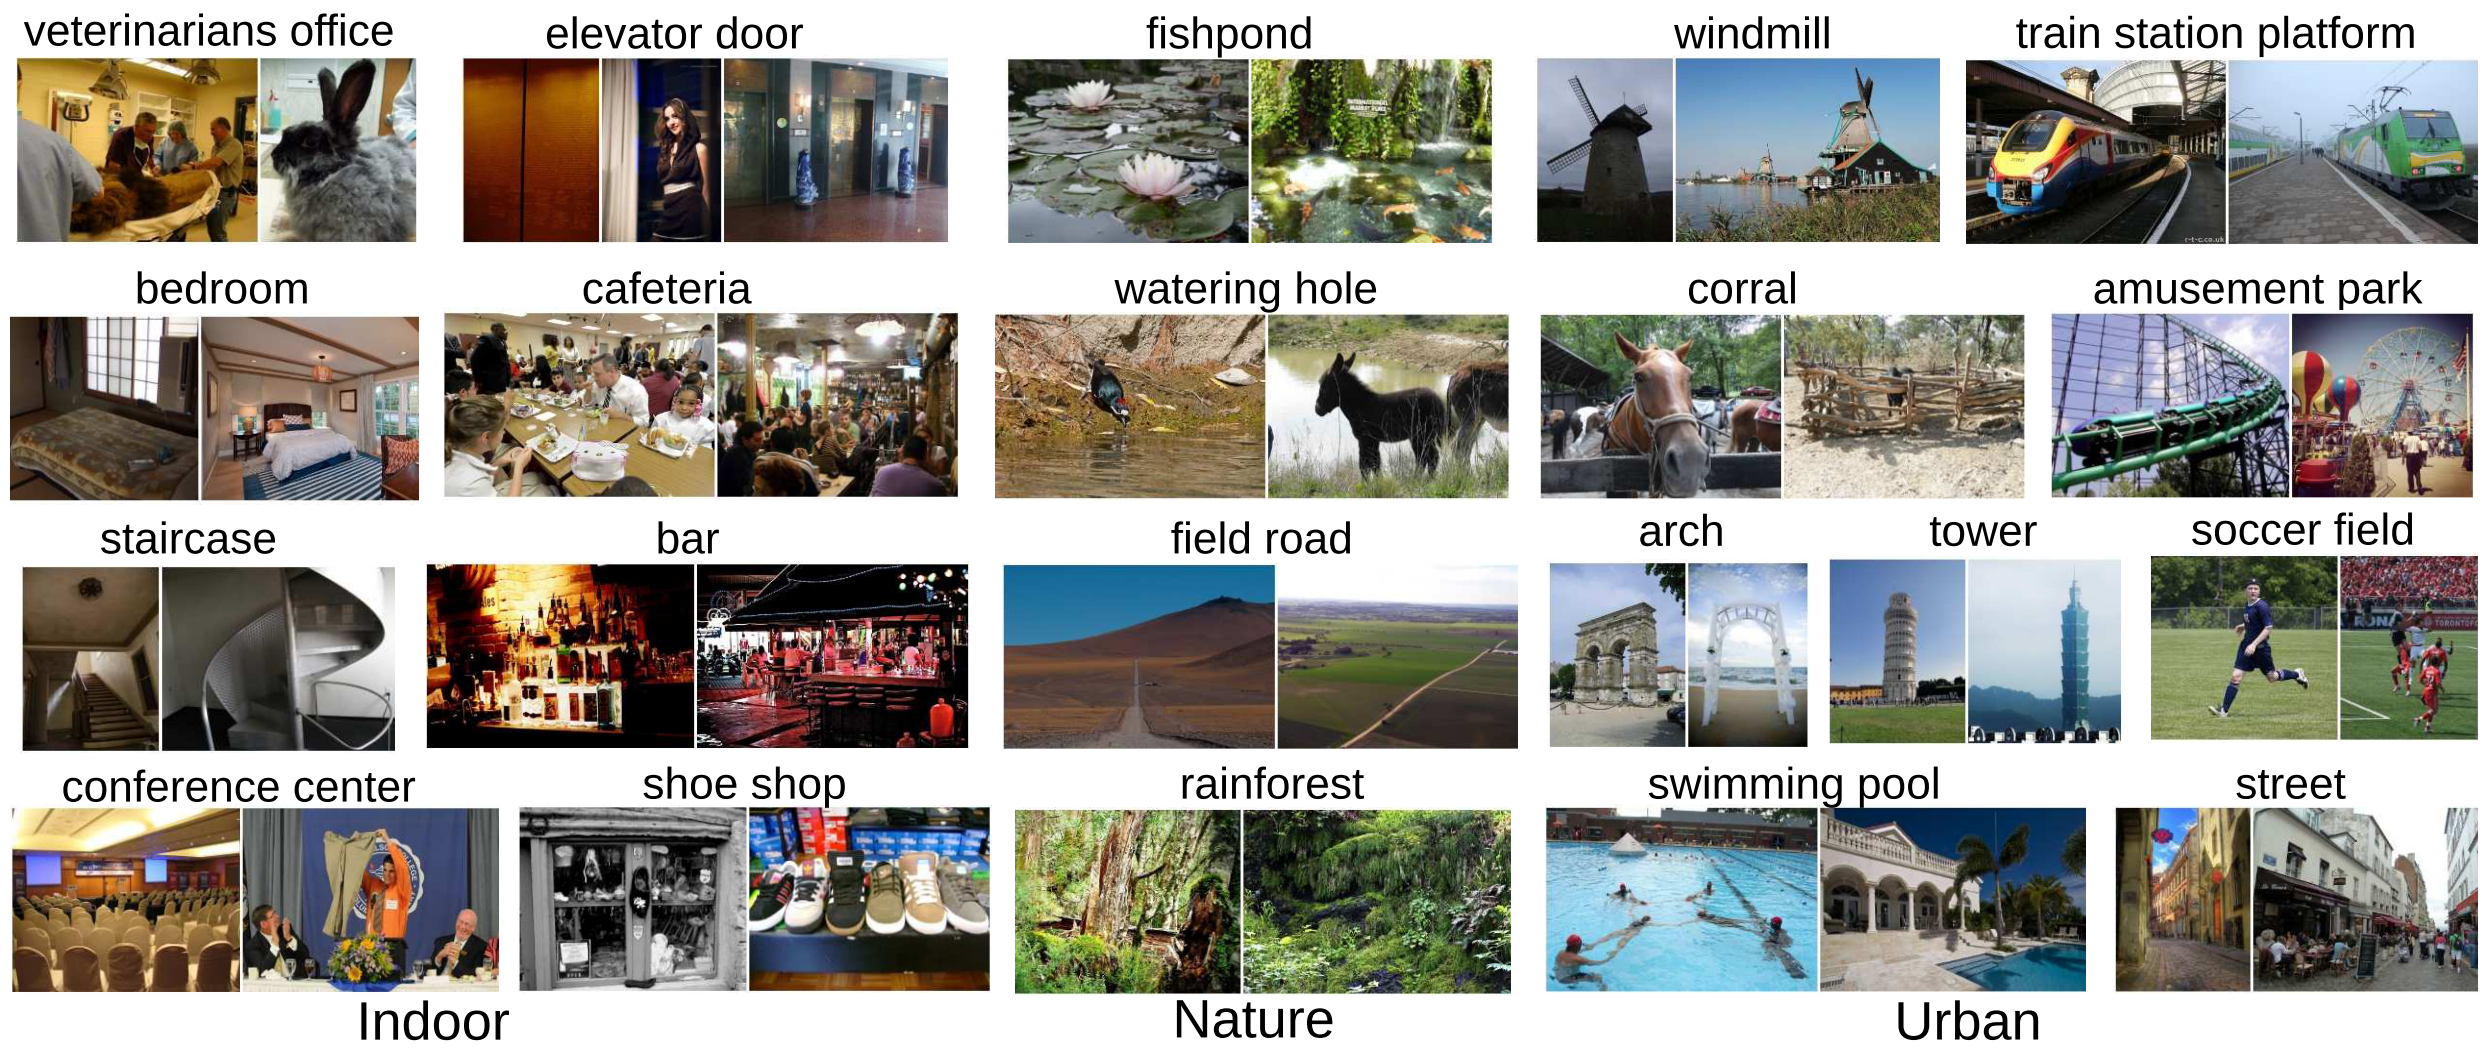
\includegraphics[scale=0.28]{pictures/random/placesart_1}
    \caption{Places macro-classes. Image source: \autocite{Places365}}
    \label{fig:placesdata1}
\end{figure}

A model trained on places should learn significantly different features from a model trained on ImageNet due to the more focused objective of the underlying data.
In particular the features it could learn from the indoor scenes may be much more adaptable to the danish housing domain.
\begin{figure}[H]
    \centering
    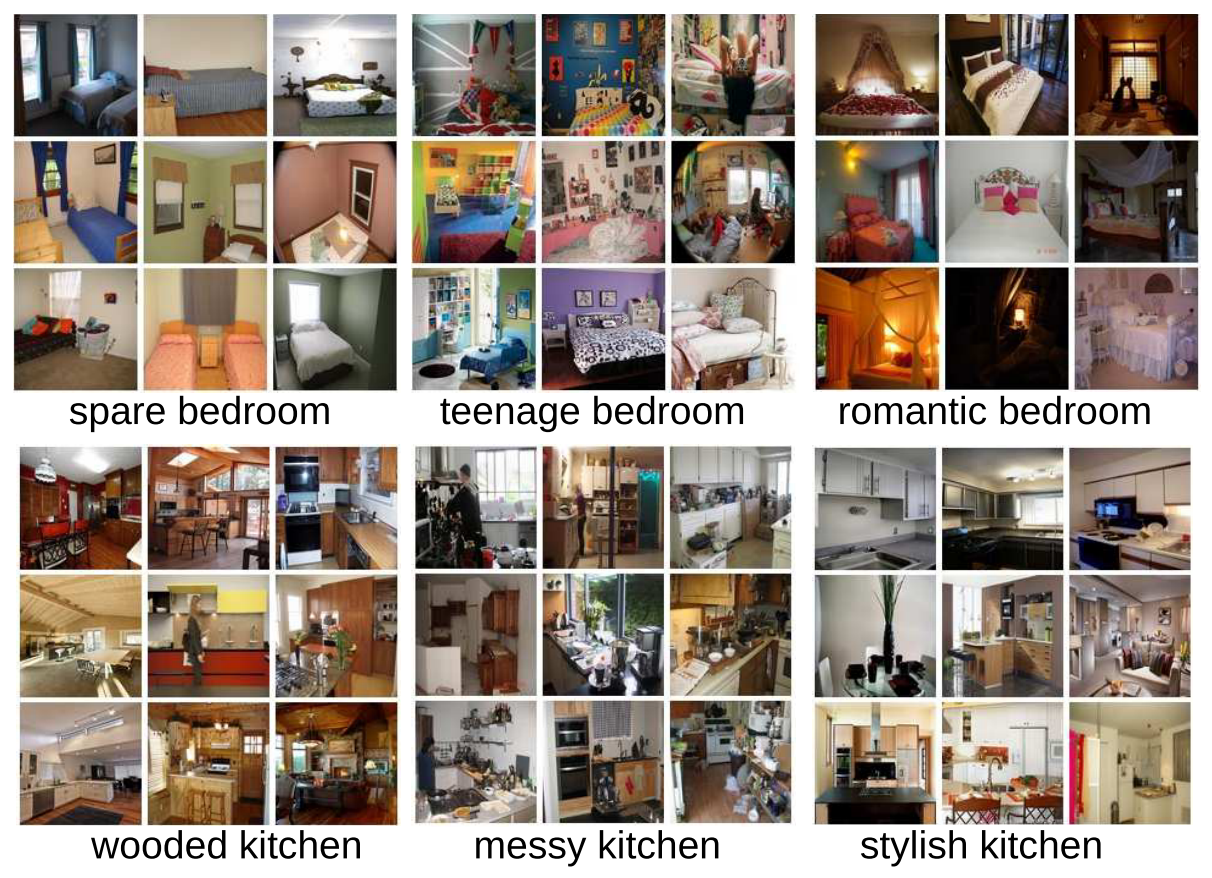
\includegraphics[scale=0.4]{pictures/random/placesart_2}
    \caption{Places indoor scene categories. Image source: \autocite{Places365}}
    \label{fig:placesdata2}
\end{figure}